\clearpage
\partsection{B-08}{Live browser checks}
\label{ev:browser}
\textbf{Manual browser walkthrough.}
The report session exercised the deployed web UI on 24 November 2026 at 18:35--18:36 UTC (25 November, 01:35--01:36 ICT). The version page reported \texttt{c32e645}, matching the full SHA for \revision{} in B-06 on p.~\pageref{ev:deploy}. The requester \texttt{req.anan} submitted a fresh synthetic 250.00 THB travel claim, \texttt{CLM-2026-000024}, assigned to \texttt{rev.malee}.

The owner opened the submitted claim and saw its details without Approve or Reject controls. The unassigned reviewer \texttt{rev.somchai} opened the same claim URL and got 403 from the claim detail request. The UI displayed the access denial without showing the claim. Both checks passed before any decision was made.

\begin{figure}[H]
  \centering
  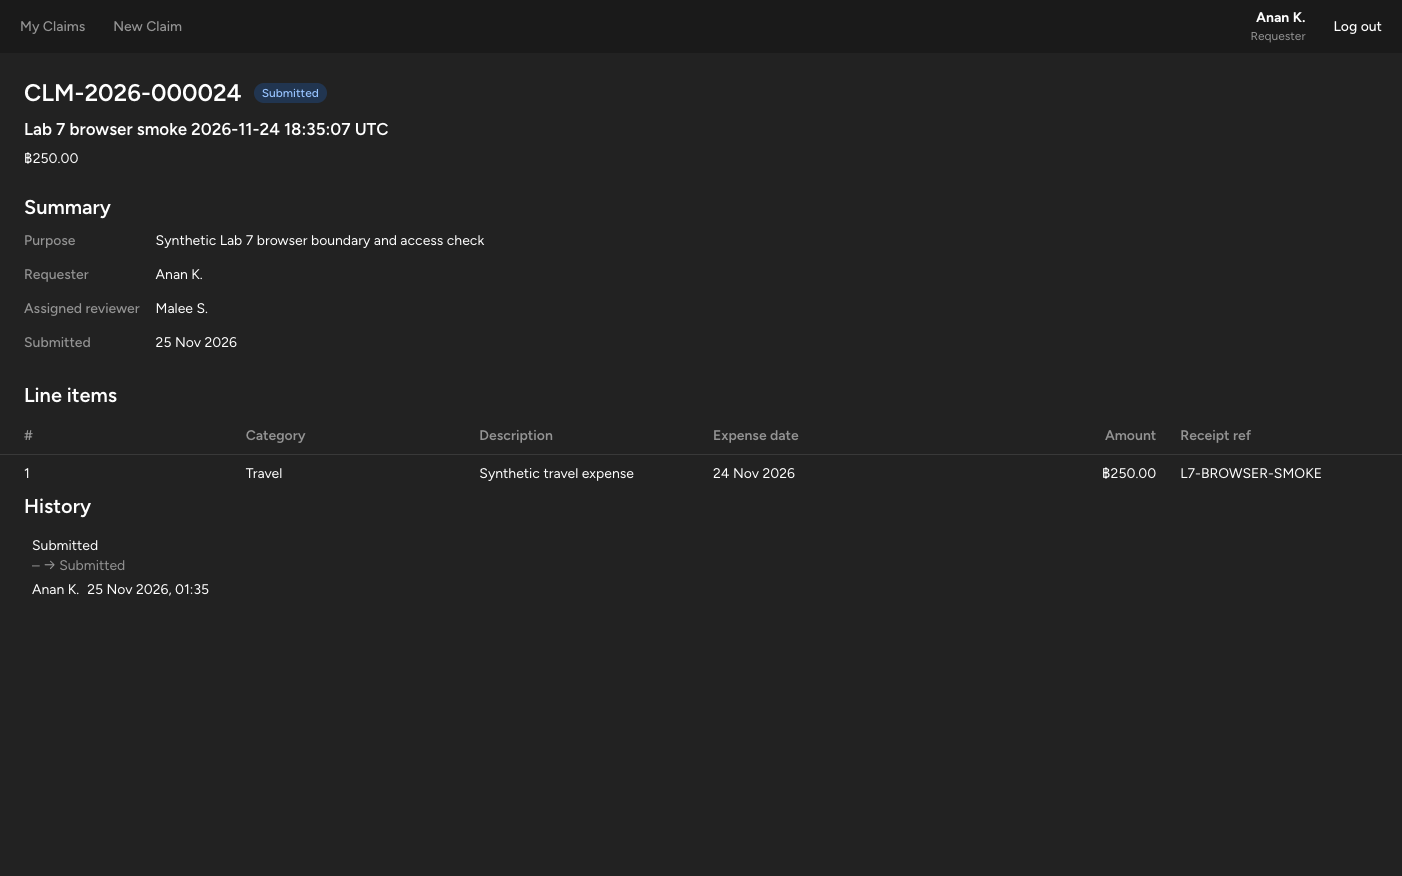
\includegraphics[width=0.96\linewidth,trim=0bp 250bp 0bp 0bp,clip]{figures/deploy/01-owner-submitted.png}
  \caption*{\textbf{B-08a.} The owner can read the submitted claim. The decision controls are absent.}
\end{figure}

\begin{figure}[H]
  \centering
  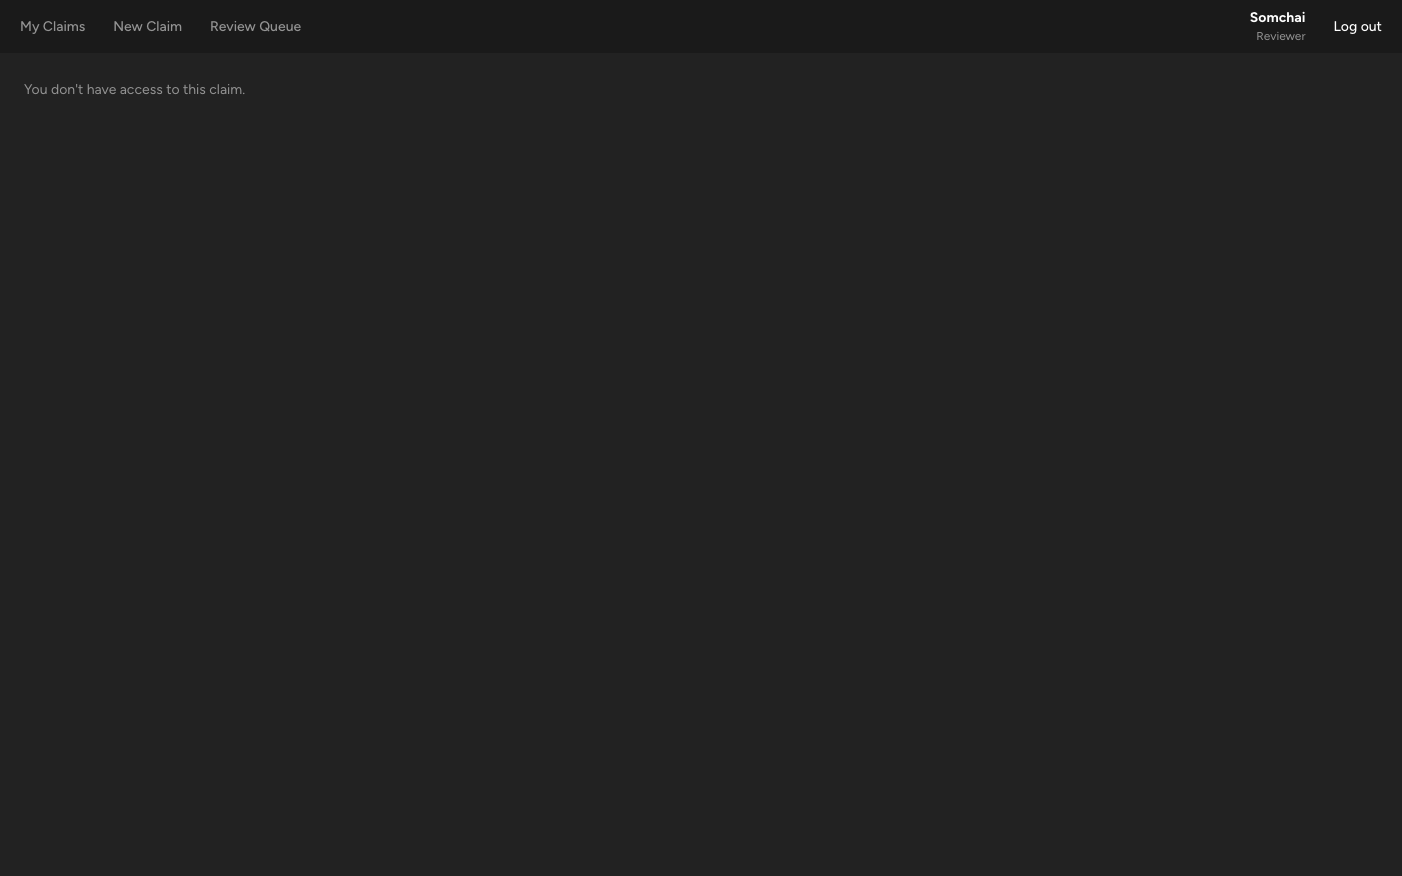
\includegraphics[width=0.96\linewidth,trim=0bp 751bp 0bp 0bp,clip]{figures/deploy/02-unassigned-reviewer.png}
  \caption*{\textbf{B-08b.} Somchai opened the same claim URL. The server returned 403 and the page displayed the denial.}
\end{figure}

\clearpage
\textbf{B-08 continued.}
Malee opened the claim from the Review Queue. An empty reason disabled Reject. Typing “No photos” showed the minimum-length message and left Reject disabled at 9. Replacing it with “No receipt” removed the inline error and enabled Reject at 10. Clicking Reject returned HTTP 200 at 18:36:27 UTC.

\begin{figure}[H]
  \centering
  \begin{minipage}[t]{0.48\linewidth}
    \centering
    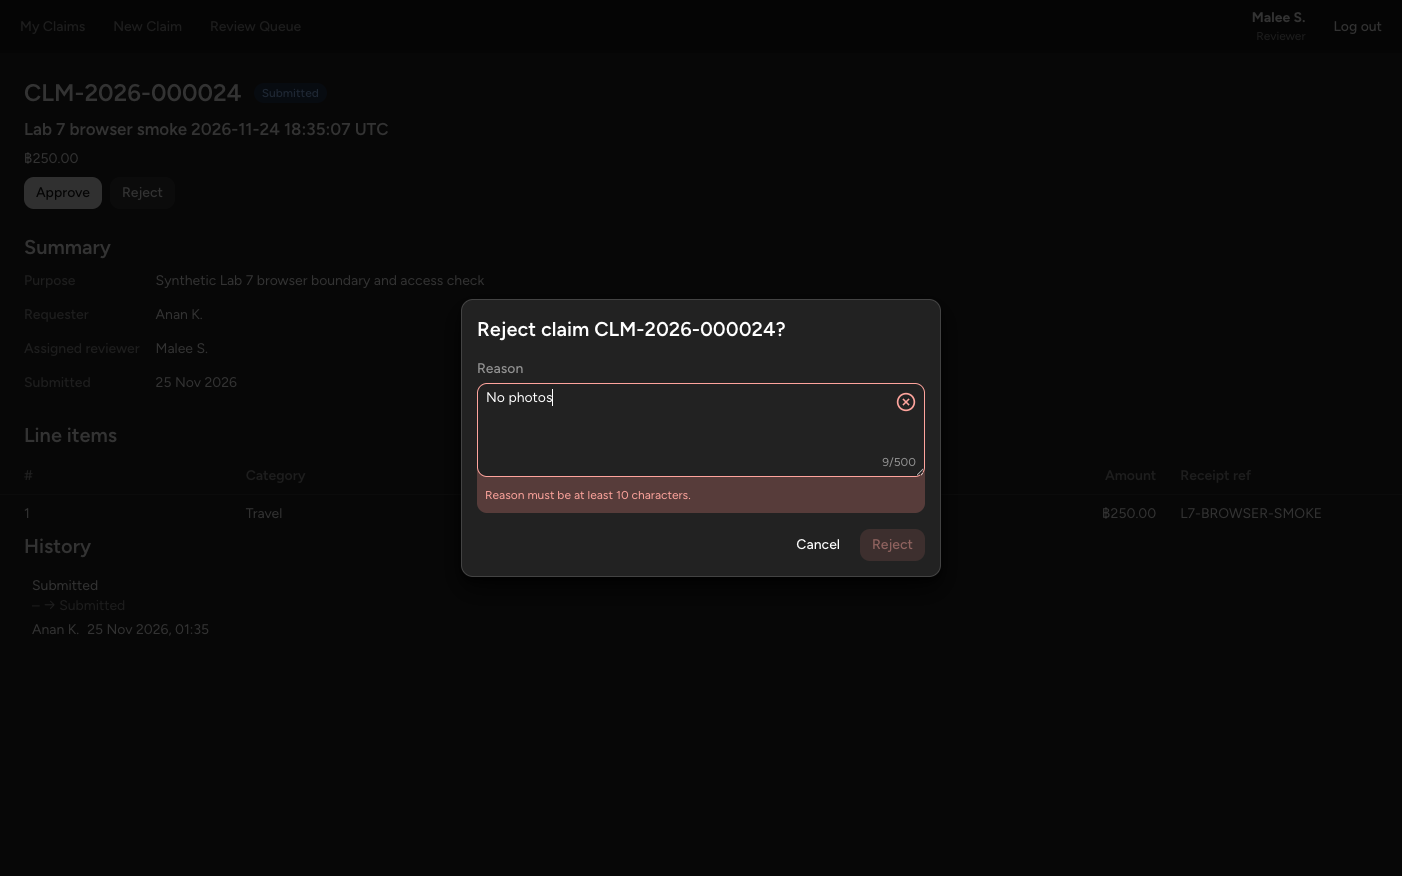
\includegraphics[width=\linewidth,trim=447bp 284bp 447bp 288bp,clip]{figures/deploy/03-reason-9.png}
    \caption*{\textbf{B-08c.} Nine characters. Reject is disabled and the field shows the minimum-length message.}
  \end{minipage}\hfill
  \begin{minipage}[t]{0.48\linewidth}
    \centering
    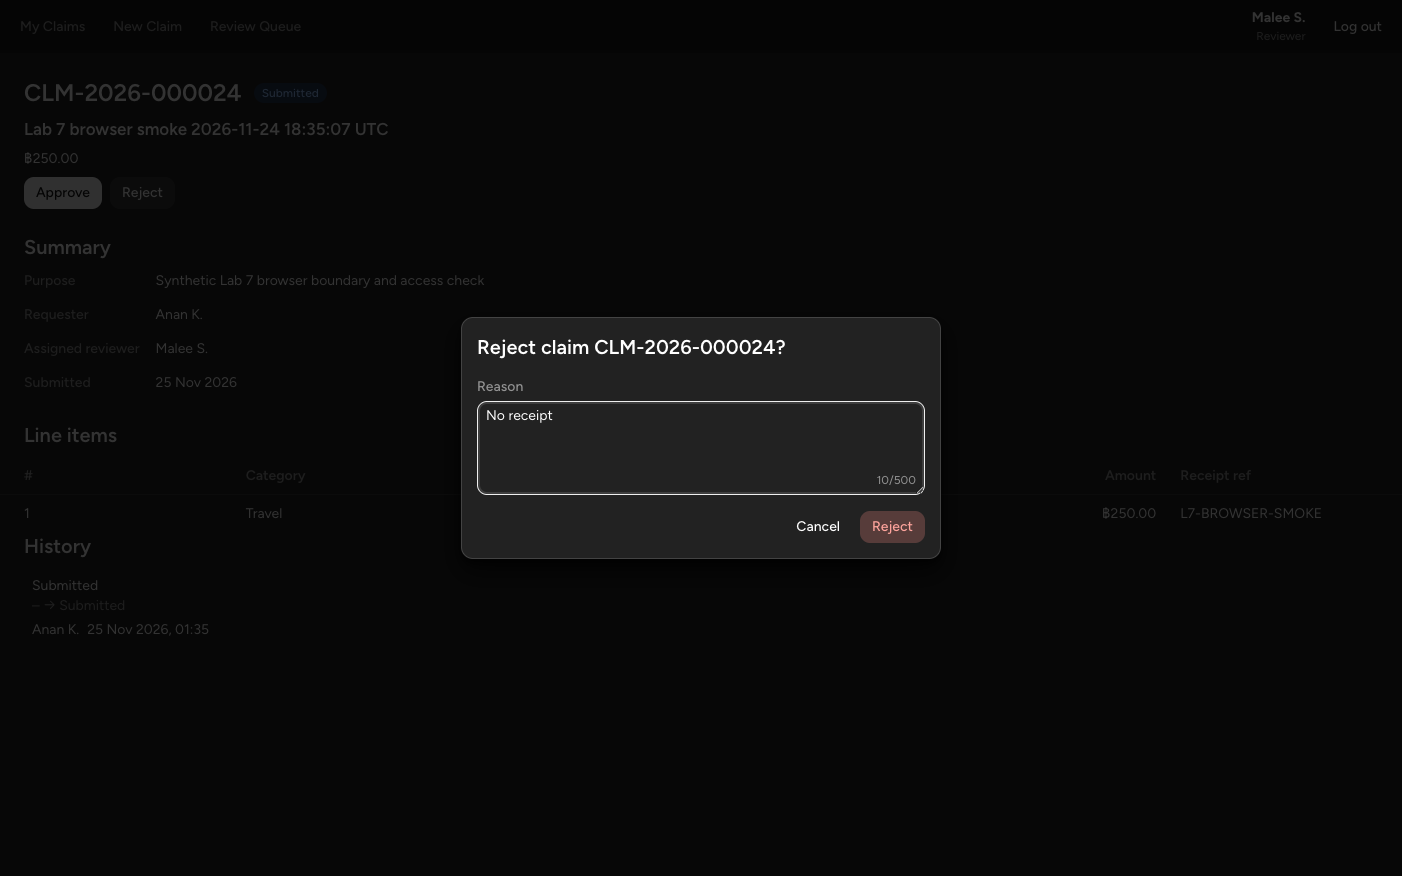
\includegraphics[width=\linewidth,trim=447bp 284bp 447bp 288bp,clip]{figures/deploy/04-reason-10.png}
    \caption*{\textbf{B-08d.} Ten characters. Reject is enabled and the inline error clears.}
  \end{minipage}
\end{figure}

The requester signed back in and opened the claim from My Claims. The status was Rejected and the history showed Malee's decision with the stored reason. All six browser checks passed. The synthetic claim remains in demo history.

\begin{figure}[H]
  \centering
  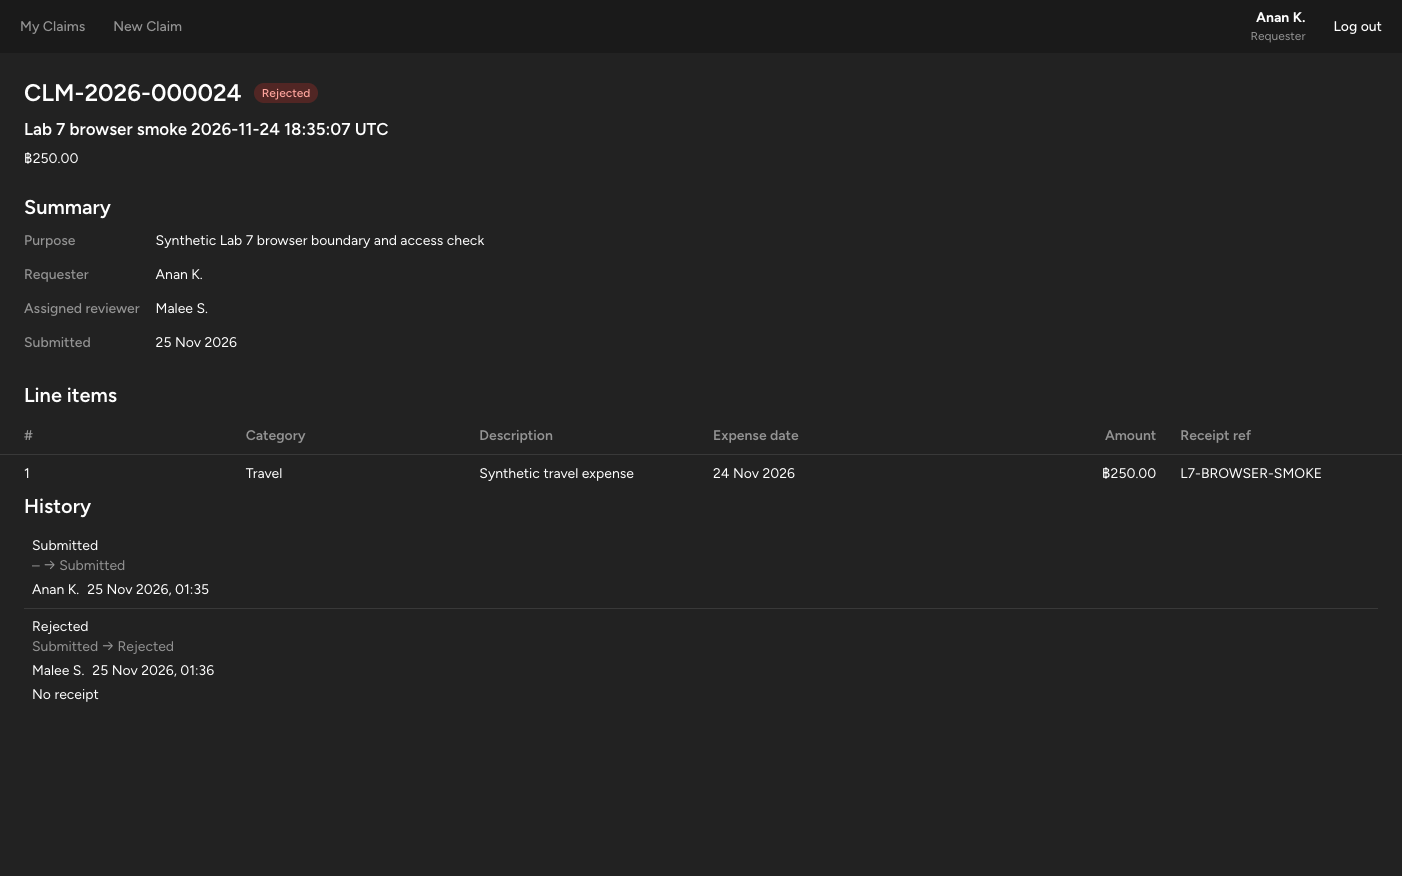
\includegraphics[width=0.96\linewidth,trim=0bp 156bp 0bp 0bp,clip]{figures/deploy/05-requester-history.png}
  \caption*{\textbf{B-08e.} The requester reopened the rejected claim and saw “No receipt” in history.}
\end{figure}
